\phantomsection

\section{Results}

Table \ref{tab:eig} shows the eigenvalues, s, determined according to four different
methods for N=400. Figure \ref{fig:plot400} shows the corresponding P (x) and U (x) eigenvectors for the highest
resolution case of each method. The eigenvectors differ only around the heat release zone, at $x = x_f = 0.25$. Main difference coming out in Galerkin method, rest of the three method showed good agreement.

\pagebreak

\begin{table}[]
	\caption{Eigenvalues, s, calculated with four different methods and, where relevant,
		up to five different resolutions, N , for the same thermoacoustic system. The growth
		rate is s r and the frequency is s i . The solutions approach each other as the resolution
		increases. (Tab comparisons.jl)}
	
	\begin{adjustbox}{width=\textwidth,center}
	\begin{tabular}{c c c c c}
		\hline \\ 
		\multicolumn{1}{c}{\textbf{N}} & \textbf{fun\_travwave}                                         & \multicolumn{1}{c}{\textbf{fun\_Helm\_FD}} & \multicolumn{1}{c}{\textbf{fun\_Helm\_FE}}   & \multicolumn{1}{c}{\textbf{fun\_Galerkin}}  \\ [3.2ex]  
		1                              & \multicolumn{1}{l}{\makecell{0.12187530859257883 \\+ 3.2227814041928715im}} & \multicolumn{1}{c}{-}                      & \multicolumn{1}{c}{-}                        & \multicolumn{1}{c}{-}                       \\ [3.2ex]
		10                             & \textbf{-}                                                     & {\makecell{0.12301472009722814 \\+ 3.2222551623591285im}} & {\makecell{1.2649666277747205e-10 \\+ 3.141592631034653im}} & {\makecell{3.42049450595866e-21 \\+ 3.1545273778453238im}} \\ [3.2ex] 
		40                             & \textbf{-}                                                     & {\makecell{0.12363155192096682 \\+ 3.221964689943754im}}  & {\makecell{0.06990252109480179 \\+ 3.184618956384646im}}    & {\makecell{0.1045690701269305 \\+ 3.2100253033952892im}}   \\ [3.2ex] 
		100                            & \textbf{-}                                                     & {\makecell{0.12115229273097906 \\+ 3.2231040481839406im}} & {\makecell{0.12302841468171331 \\+ 3.2235632383934383im}}   & {\makecell{0.12181433836201444 \\+ 3.2228598981240886im}}  \\ [3.2ex] 
		400                            & -                                                              & 
		{\makecell{0.12205739886178892 \\+ 3.2226989128574868im}} & {\makecell{0.12181867950887351 \\+ 3.2227425705073545im}}   & {\makecell{0.12181840527018106 \\+ 3.2227499047678436im}}  \\ [3.2ex]  \hline
	\end{tabular}
\end{adjustbox}


\label{tab:eig}
\end{table}


Table \ref{tab:sens} tabulates the calculated base sensitivities of each method.

\FloatBarrier
\begin{figure}[!t]
	
	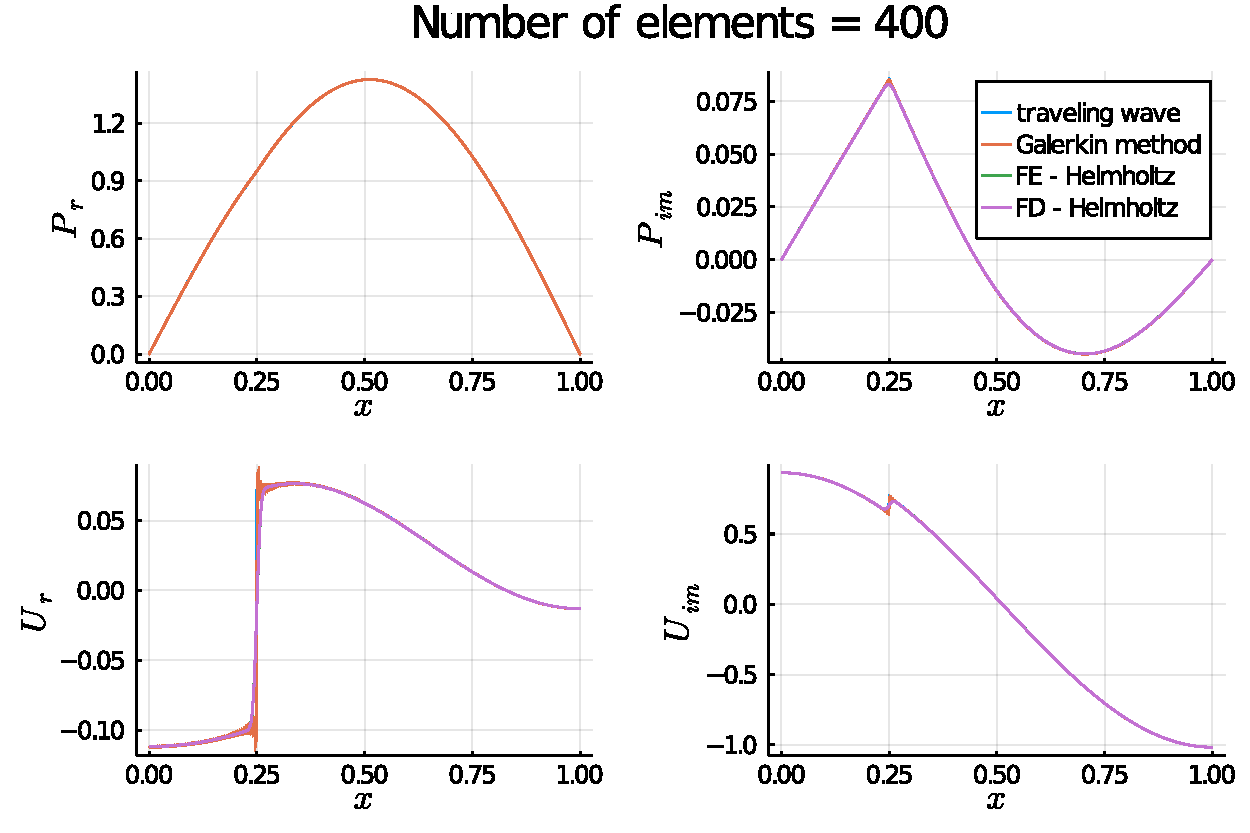
\includegraphics[width=\textwidth]{400plot.pdf}
	\caption{Real and imaginary components of the pressure, P (x), and velocity, U (x), eigenfunctions
		calculated for the highest resolution cases of the methods shown in table 1.  (Tab\_comparisons.jl)}
	\label{fig:plot400}
	
\end{figure}
\FloatBarrier

\pagebreak

\FloatBarrier
\begin{table}[ht!]
	\caption{Base state sensitivities calculated by means of four methods with N = 400 (Tab comparisons.jl)}
	\begin{adjustbox}{width=\textwidth,center}
		\begin{tabular}{lcccc}
			\hline \\ 
			\textbf{}                 & \textbf{$\partial s/\partial n$}                              & \textbf{$\partial s/\partial \tau$}                             & \textbf{$\partial s/\partial x_m$}                            & \textbf{$\partial s/\partial x_f$}                           \\ [3.2ex]
			\textbf{fun\_travwave.jl} & {\makecell{0.10298315656272834 \\+ 0.08269441085108045im}} & {\makecell{0.2539549055356268 \\- 0.34197060875680085im}} & {\makecell{-0.2664856896104548 \\- 0.17766984877202488im}}  & {\makecell{0.43129016791308405 \\+ 0.21134136333692508im}} \\ [3.2ex]
			\textbf{fun\_Helm\_FD.jl} & {\makecell{0.1029381172495191 \\+ 0.08265540766612185im}}  & {\makecell{0.2538373154537853 \\- 0.341812025204056im}}   & {\makecell{-0.2663486625117436 \\- 0.17759310185260918im}}  & {\makecell{0.4310431667740005 \\+ 0.2112708145173602im}}   \\ [3.2ex]
			\textbf{fun\_Helm\_FE.jl} & {\makecell{0.10293804348656137 \\+ 0.08265471643133453im}} & {\makecell{0.2538357312085307 \\- 0.34181243558702773im}} & {\makecell{-0.2663469127817901 \\- 0.17759196026029755im}}  & {\makecell{0.4310398326117469 \\+ 0.21126935565722768im}}  \\ [3.2ex]
			\textbf{fun\_Galerkin.jl} & {\makecell{0.1033169131009024 \\+ 0.08257175330986924im}}  & {\makecell{0.253493305952927 \\- 0.3430377969585296im}}   & {\makecell{-0.26685205730784367 \\- 0.17749521966955883im}} & {\makecell{0.398800858731003 \\+ 0.2259008693655126im}} \\ [3.2ex]  \hline   
		\end{tabular}
	\end{adjustbox}
\label{tab:sens}
\end{table}
\FloatBarrier


